\documentclass{stdlocal}
\begin{document}
\section{SIMD-Capable Processors} % (fold)
\label{sub:simd-capable_processors}

  According to \textcite[\ppno~10-11]{hennessy2019}, in the year 1966, Flynn classified parallel architectures of computers with respect to their data-level and task-level parallelism.
  Based on this classification, a conventional uniprocessor has a single instruction stream and single data stream, also known as single instruction single data (SISD) architecture \autocite[\ppno~509-510]{patterson2014}.
  The single instruction multiple data (SIMD) architecture exploits data-level parallelism by applying the same operations to multiple items of independent data at the same time \autocite{hennessy2019} which, from the programmer's perspective, is close to the SISD mode of operation \autocite{patterson2014}.
  In contrast to the multiple instruction multiple data (MIMD) architecture, SIMD only has to fetch one instruction to launch several data operations potentially reducing the power consumption.
  The application of SIMD ranges from matrix-oriented algorithms in scientific computing to media-oriented image and sound processing, as well as machine learning algorithms \autocite[\ppno~10-11]{hennessy2019}.
  Modern Intel processors typically provide SIMD utilities through special vector registers and a richer instruction set, like the Streaming SIMD Extensions (SSE) and the Advanced Vector Extensions (AVX) \autocite{intel-intrinsics-guide,fog2019a,fog2019b,fog2019c,fog2019d,fog2019e}.
  At the same time, MIMD utilities are implemented through multiple processor cores and multithreading.
  In a modern processor, SIMD and MIMD are orthogonal features of its design and can therefore be discussed independently.
  Hence, we will not focus on the exploitation of the MIMD architecture.
  To be able to design and implement vectorized algorithms for an SIMD architecture, we have to explain how data-level and instruction-level parallelism can be used to raise the performance of a computer program.
  % Vectorization techniques can be conceptualized by the architecture of modern SIMD-capable multiprocessors and their instruction sets.
  Especially the knowledge of typical instructions will make the design of a new API and its application to Monte Carlo simulations clear.
  Therefore, we will briefly introduce the fundamentals of computer architecture and refer to \textcite{patterson2014} and \textcite{hennessy2019} for a more detailed observation.
  In reality, there are several different SIMD-capable CPU architectures.
  Here, we will restrict our discussions to the SSE and AVX instruction set architectures from modern Intel processors, like the \citetitle{intel-kaby-lake-i7} and the \citetitle{intel-kaby-lake-i5} used to test implementations of described PRNGs \autocite{intel-kaby-lake-i5,intel-kaby-lake-i7}.

  \subsection{Fundamentals of Computer Architecture}
    The Von Neumann architecture still describes the basic organization of a modern computer.
    Besides external mass storage, like hard disk drives (HDDs), and input/output (IO) mechanisms, the model consists of two main parts --- the central processing unit (CPU), also called the processor, to execute instructions from a computer program, and the memory to store the respective data and instructions \autocite{hennessy2019}.
    Today, both, data and instructions, are encoded as binary numbers with fixed length which has proven to make the building and functioning of a computer much more efficient \autocite{patterson2014}.

    \subsubsection*{The Processor}
    \begin{figure}
      \center
      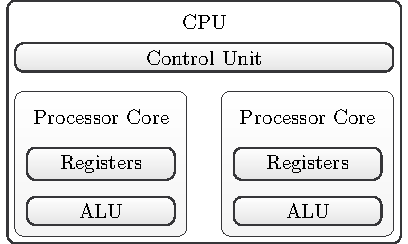
\includegraphics[width=0.5\textwidth]{figures/cpu_components.pdf}
      \caption[Hierarchical Order of CPU Components]{%
        The figure shows the basic components of a typical CPU with multiple processing cores in an hierarchical order.
        There is only one control unit which is handling communication between different cores by coordinating the execution of program instructions.
        Every processor core employs its own registers and ALUs to provide an MIMD architecture.
      }
      \label{fig:cpu-components}
    \end{figure}
    The processor in general consists of multiple arithmetic logic units (ALU) or execution units, a small number of registers and a control unit.
    The ALU performs arithmetic and logic operations and stores its results in registers.
    These registers also supply the operands for ALU operations.
    To fetch program instructions from memory and executing them, the control unit directs the coordinated operations of the ALU, registers and other components.
    Today, nearly every processor consists even of multiple processing cores each connected by a global control unit and containing its own registers and ALUs to provide an MIMD architecture.
    In figure \ref{fig:cpu-components}, all the named components are shown schematically in a hierarchy to support the understanding.
    Here, we will focus on a single processing core.

    The set of instructions a CPU is able to execute is called its architecture.
    Usually, processor architectures provide commands to move data between memory and registers and simple arithmetic and logic operations, like addition and multiplication of integral or floating-point numbers, to actually compute results of algorithms.
    The actual implementation of an instruction set in form of a processor circuit is called the microarchitecture.
    It defines how instructions are executed in reality by providing different execution units and modes of operation.
    Hence, with respect to the microarchitecture instructions suddenly exhibit physical properties, like the time to execute the given instruction, that were not considered by the abstract processor architecture.
    \autocite{hennessy2019,patterson2014}

    Executing an instruction in the processor is done in several stages.
    The number and kind of these stages depend on the type of the instruction and the underlying microarchitecture of the CPU.
    For example, an instruction first has to be fetched from memory.
    Afterwards, the bits of the instruction will be decoded and all referenced registers will be read.
    Finally, the ALU computes the actual operation and stores the result in the target register.
    Basically we can say, each stage is completed after one CPU cycle.
    The number of CPU cycles an instruction needs to be finished and provide its result to the next instruction is called its latency.
    The throughput of an instruction is measured in cycles per instruction and specifies the number of cycles an instruction needs to reside in the execution unit.

    To speed up the execution of independent instructions, in nearly all modern CPUs a so-called pipeline is used.
    Independent instructions do not have to wait for the results of other immediate instructions and therefore do not need to stall the execution unit for their complete latency.
    Instead, the processor is performing the different stages of different instructions concurrently according to their throughput.
    For a better understanding, figure \ref{fig:pipeline} shows a schematic example of this pipeline process for four independent instructions with a latency of four and a throughput of one.
    As a consequence, a pipeline does not reduce the latency of an instruction but increases its throughput.
    It is therefore a form of instruction-level parallelism.
    To further decrease the throughput of instructions, the processor core typically uses multiple execution units to run independent instructions directly in parallel.
    This enhancement is shown in figure \ref{fig:multiple-unit-pipeline} with eight independent again with a latency of four and a throughput of one.

    \begin{figure}
      \center
      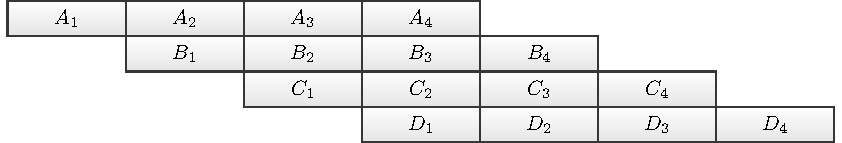
\includegraphics[width=0.95\textwidth]{figures/pipeline.pdf}
      \caption[Pipeline Structure]{%
        This figure shows the functioning of a pipeline.
      }
      \label{fig:pipeline}
    \end{figure}
    The theoretical performance of the CPU pipeline is reduced if it has to be stalled.
    These situations, also known as hazards, happen due to hardware resource conflicts, data dependencies and control instructions, like branches.
    To handle control instructions and especially branches much more efficiently, the CPU uses branch prediction.
    The processor tries to guess the outcome of the branch condition to keep the pipeline filled.
    Should the estimated value proven to be wrong the pipeline has to be stalled and cleared.
    This process is called a branch miss and introduces an execution time penalty.
    Hence, we will strive for branchless code or for easy-to-predict branches if we have to insert them.
    \begin{figure}
      \center
      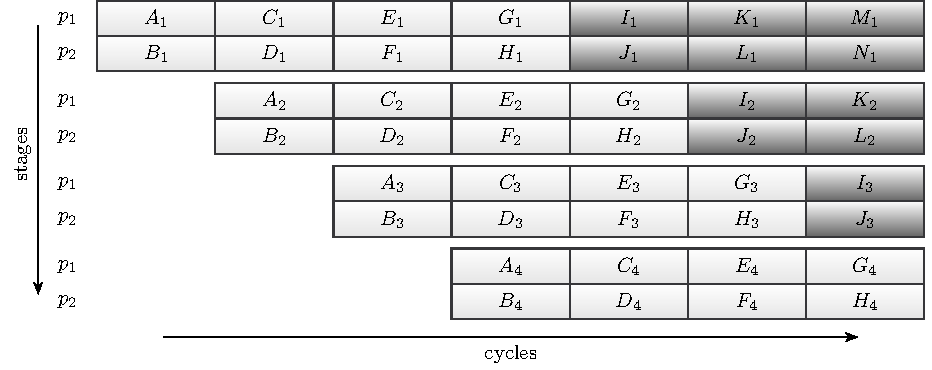
\includegraphics[width=0.95\textwidth]{figures/multiple_unit_pipeline.pdf}
      \caption[Multiple Unit Pipeline Structure]{%
        This figure shows the functioning of a pipeline.
      }
      \label{fig:multiple-unit-pipeline}
    \end{figure}

    For data-level parallelism, we want to focus on SIMD architectures.
    Intel CPUs establish this feature by using so-called vector registers of a fixed length.
    Vector registers contain more than one value at the same time.
    For example, a $256\appendUnit{bit}$ register can contain four $64\appendUnit{bit}$ values or eight $32\appendUnit{bit}$ values.
    One operation, like addition or multiplication, is then performed on all contained elements simultaneously.
    The choice which pattern to use is based on the trade-off between precision and throughput.
    If an application demands a high precision from the underlying floating-point operations, it will be more efficient to use four $64\appendUnit{bit}$ double precision values reducing the throughput instead of eight single precision values.

    \subsubsection*{The Memory}
    Memory can be described as a finite sequence of bits, whereby each bit anytime represents either the value $0$ or $1$.
    Eight bits are grouped into a byte and enumerated with a natural number starting from zero.
    These numbers are called memory addresses and make it possible to specify the location of variables in memory.
    This basic interpretation is visualized in figure \ref{fig:memory}.
    Fetching instructions from memory or transferring data between the CPU and memory, therefore requires the usage of those memory addresses to be able to reference data in the sequence of bytes.
    Each byte can be altered by program execution through storing instructions.
    \autocite{patterson2014}
    \begin{figure}[H]
      \center
      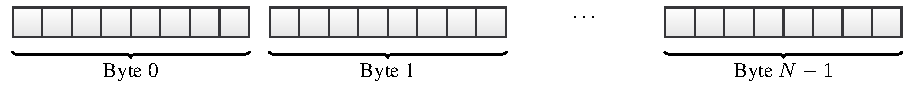
\includegraphics[width=0.95\textwidth]{figures/memory.pdf}
      \caption[Memory Structure]{%
        This figure visualizes memory with $N\in\setNatural$ bytes as a sequences of bits where each byte can be referenced by its memory address.%
      }
      \label{fig:memory}
    \end{figure}
    Because physically there is no possibility to provide an unlimited amount of fast memory, computer designers found a more economical solution.
    In the majority of cases, faster memory means reduced storage capabilities and vice versa.
    Hence, memory is built to be a hierarchy of several levels --- each smaller, faster, and more expensive per byte than the next lower level, which is farther from the processor.
    Interleaving levels are called caches and with caching we mean the process of loading data into the next cache level.
    If the processor wants to load some data from memory which cannot be found in the first level cache, data has to be fetched from a lower level in the hierarchy.
    This is called a cache miss.
    If on the other hand the data can be found in the cache, it can be directly used by the higher level cache or the processor itself.
    We call this a cache hit.
    A cache miss introduces a so-called miss penalty to the memory access time and should therefore be avoided to reduce the latency for fetching instructions and data.
    Figure \ref{fig:memory-hierarchy} shows a schematic view of a usual memory hierarchy found in today's laptops and desktop computers.
    In modern processor architectures, like the Kaby Lake microarchitecture from Intel, each processing core of the CPU features its own level one cache which is further split into an instruction cache and a data cache \autocite{intel-kaby-lake}.
    This reduces the overall complexity of level one caches and as a result decreases the cache access time.
    \autocite[\ppno~78-83]{hennessy2019}
    \begin{figure}
      \center
      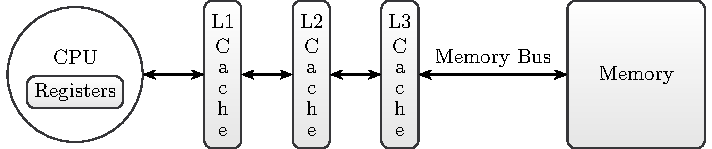
\includegraphics[width=0.95\textwidth]{figures/memory_hierarchy.pdf}
      \caption[Memory Hierarchy Scheme]{%
        The figure shows a scheme of the non-persistent part of the memory hierarchy for a modern laptop or desktop computer.
        Modeled after \textcite[\pno~79]{hennessy2019}.
      }
      \label{fig:memory-hierarchy}
    \end{figure}

    % The size in bytes of a simple variable in memory can be expressed by a power of two.
    % In C++ for example, single and double precision floating-point numbers, as well as signed and unsigned integers fulfill this requirement.
    Let $n \define 2^k$ for some $k\in\setNatural_0$ be a power of two.
    We say that a variable in memory is $n\appendUnit{Byte}$ aligned if its starting address is divisible by $n$ without remainder.
    Modern systems typically provide a $16\appendUnit{Byte}$ alignment as default.
    SSE vector registers have a size of $128\appendUnit{bit}$ and even demand that variables to be loaded from memory exhibit a $16\appendUnit{Byte}$ alignment.
    The AVX architecture of Intel CPUs is working with $256\appendUnit{bit}$ or $32\appendUnit{Byte}$ long vector registers which do not have to be aligned but should provide a slightly improved performance otherwise.
    \autocite{fog2019a}

  \subsection{Usage in C++} % (fold)
  \label{sub:usage_in_c_}
    To force the usage of the SSE or AVX instructions which exploit the SIMD capabilities on modern Intel processors, assembler code resulting from compiling a given program has to explicitly call the according instructions of the microarchitecture.
    To achieve this behavior in C++, there are several variants.

    First, we could use inline assembly code to directly call the appropriate instructions.
    This was done in \textcite{guskova2016,barash2017}.
    But developing modules with inline assembly statements tends to be error-prone, complicated, unmaintainable and often results in code bloat.

    The second variant uses the automatic vectorization of the compiler.
    Typically, this process should be preferred in contrast to manually optimizing the code by introducing SSE or AVX instructions to provide machine independent code.
    Due to the compiler's knowledge of the underlying hardware, automatic vectorization often generates code that is superior to other variants.
    But sometimes the complexity of problems exhibits several data and instruction dependencies by using non-trivial branches with different code paths or long chains of dependent calculations.
    In such cases, the compiler will not be able vectorize the code and we as programmers have to fall back to a manual alternative.

    To get the best of both worlds, Intel provides so-called SIMD intrinsics for the SSE and AVX instruction sets.
    Theses intrinsics describe abstract functions in the C++ language working with data types representing vector registers and are not defined by the language itself.
    Each intrinsic is basically substituting an assembler instruction.
    With these utilities, it is possible to manually vectorize the code without the need to use inline assembly statements.
    Therefore, we are able to use high-level abstraction features of C++ to create a usable API and make the code maintainable while inserting low-level routines to improve its performance.
    Usually, this approach is easier to understand, less error-prone and results in less code than inline assembly statements.
    Above all, taking care of alignment, latency and throughput of operations is made much simpler due to the abstraction of registers to variables.
    The latencies and throughputs of specific intrinsics for different microarchitectures is given by \textcite{intel-intrinsics-guide} and \textcite{fog2019d}.
    As a consequence, we rely on this variant to develop the vectorized implementations of PRNGs and algorithms.

    The AVX intrinsic data types are given by \texttt{\_\_m256}, \texttt{\_\_m256d}, \texttt{\_\_m256i} representing eight single precision floating-point values, four double precision floating-point values and a different amount of integer numbers with different sizes.
    The name of each intrinsic is based on the same pattern which first encodes the instruction set to use, followed by the code name of the operation, finished by identification of the storage pattern all separated by underscores.
    The SSE instruction set is encoded by \texttt{\_mm} and the AVX instruction set by \texttt{\_mm256}.
    For example, the name of the AVX intrinsic to add every element of two other vectors each containing eight single precision floating-point values is given by \texttt{\_mm256\_add\_ps}.
  % subsection usage_in_c_ (end)
% section simd-capable_processors (end)
\end{document}